\documentclass{article}

% packages
\usepackage{amsmath, amsthm, thmtools, amsfonts, amssymb, luacode, catchfile, tikzducks, hyperref, ifthen}
\ifcsname c@kobocompile\endcsname
	\usepackage[a5paper, total={1072pt, 1448pt}, margin=10pt, includeheadfoot]{geometry} % set page margins
\else
	\usepackage[a4paper, margin=50pt, includeheadfoot]{geometry}
\fi
\usepackage[shortlabels]{enumitem}
\usepackage[skip=3pt, indent=0pt]{parskip}

% language
\usepackage[bidi=basic, layout=tabular, provide=*]{babel}
\ifcsname c@english\endcsname
	\babelprovide[main, import]{english}
\else
	\babelprovide[main, import]{hebrew}
	\babelprovide{rl}
\fi
%\babelfont{rm}{Libertinus Serif}
\babelfont{rm}[Renderer=Harfbuzz]{Libertinus Serif}
\babelfont{sf}{Libertinus Sans}
\babelfont{tt}{Libertinus Mono}

% style
\AddToHook{cmd/section/before}{\clearpage}	% Add line break before section
\linespread{1.3}
\setcounter{secnumdepth}{0}		% Remove default number tags from sections, this won't do well with theorems
\AtBeginDocument{\setlength{\belowdisplayskip}{3pt}}
\AtBeginDocument{\setlength{\abovedisplayskip}{3pt}}
\graphicspath{ {../images/} }

% operators
\DeclareMathOperator\cis{cis}
\DeclareMathOperator\Sp{Sp}
\DeclareMathOperator\tr{tr}
\DeclareMathOperator\im{Im}
\DeclareMathOperator\re{Re}
\DeclareMathOperator\diag{diag}
\DeclareMathOperator*\lowlim{\underline{lim}}
\DeclareMathOperator*\uplim{\overline{lim}}
\DeclareMathOperator\rng{rng}
\DeclareMathOperator\Sym{Sym}
\DeclareMathOperator\Arg{Arg}
\DeclareMathOperator\Log{Log}
\DeclareMathOperator\dom{dom}
\DeclareMathOperator\supp{Supp}
\DeclareMathOperator\var{Var}
\DeclareMathOperator\cov{Cov}

% commands
%\renewcommand\qedsymbol{\textbf{מש''ל}}
%\renewcommand\qedsymbol{\fbox{\emoji{lizard}}}
\newcommand{\Aa}[0]{\mathcal{A}}
\newcommand{\Bb}[0]{\mathcal{B}}
\newcommand{\CC}[0]{\mathbb{C}}
\newcommand{\Cc}[0]{\mathcal{C}}
\newcommand{\EE}[0]{\mathbb{E}}
\newcommand{\FF}[0]{\mathbb{F}}
\newcommand{\Ff}[0]{\mathcal{F}}
\newcommand{\Ii}[0]{\mathcal{I}}
\newcommand{\Gg}[0]{\mathcal{G}}
\newcommand{\Ll}[0]{\mathcal{L}}
\newcommand{\Mm}[0]{\mathcal{M}}
\newcommand{\NN}[0]{\mathbb{N}}
\newcommand{\Nn}[0]{\mathcal{N}}
\newcommand{\PP}[0]{\mathbb{P}}
\newcommand{\Pp}[0]{\mathcal{P}}
\newcommand{\QQ}[0]{\mathbb{Q}}
\newcommand{\RR}[0]{\mathbb{R}}
\newcommand{\Rr}[0]{\mathcal{R}}
\newcommand{\Ss}[0]{\mathcal{S}}
\newcommand{\TT}[0]{\mathbb{T}}
\newcommand{\Uu}[0]{\mathcal{U}}
\newcommand{\Vv}[0]{\mathcal{V}}
\newcommand{\Ww}[0]{\mathcal{W}}
\newcommand{\ZZ}[0]{\mathbb{Z}}
\newcommand{\acts}[0]{\circlearrowright}
\newcommand{\explain}[2] {
	\begin{flalign*}
		 && \text{#2} && \text{#1}
	\end{flalign*}
}
\newcommand{\maketitleprint}[0]{ \begin{center}
	%\begin{tikzpicture}[scale=3]
	%	\duck[graduate=gray!20!black, tassel=red!70!black]
	%\end{tikzpicture}	
	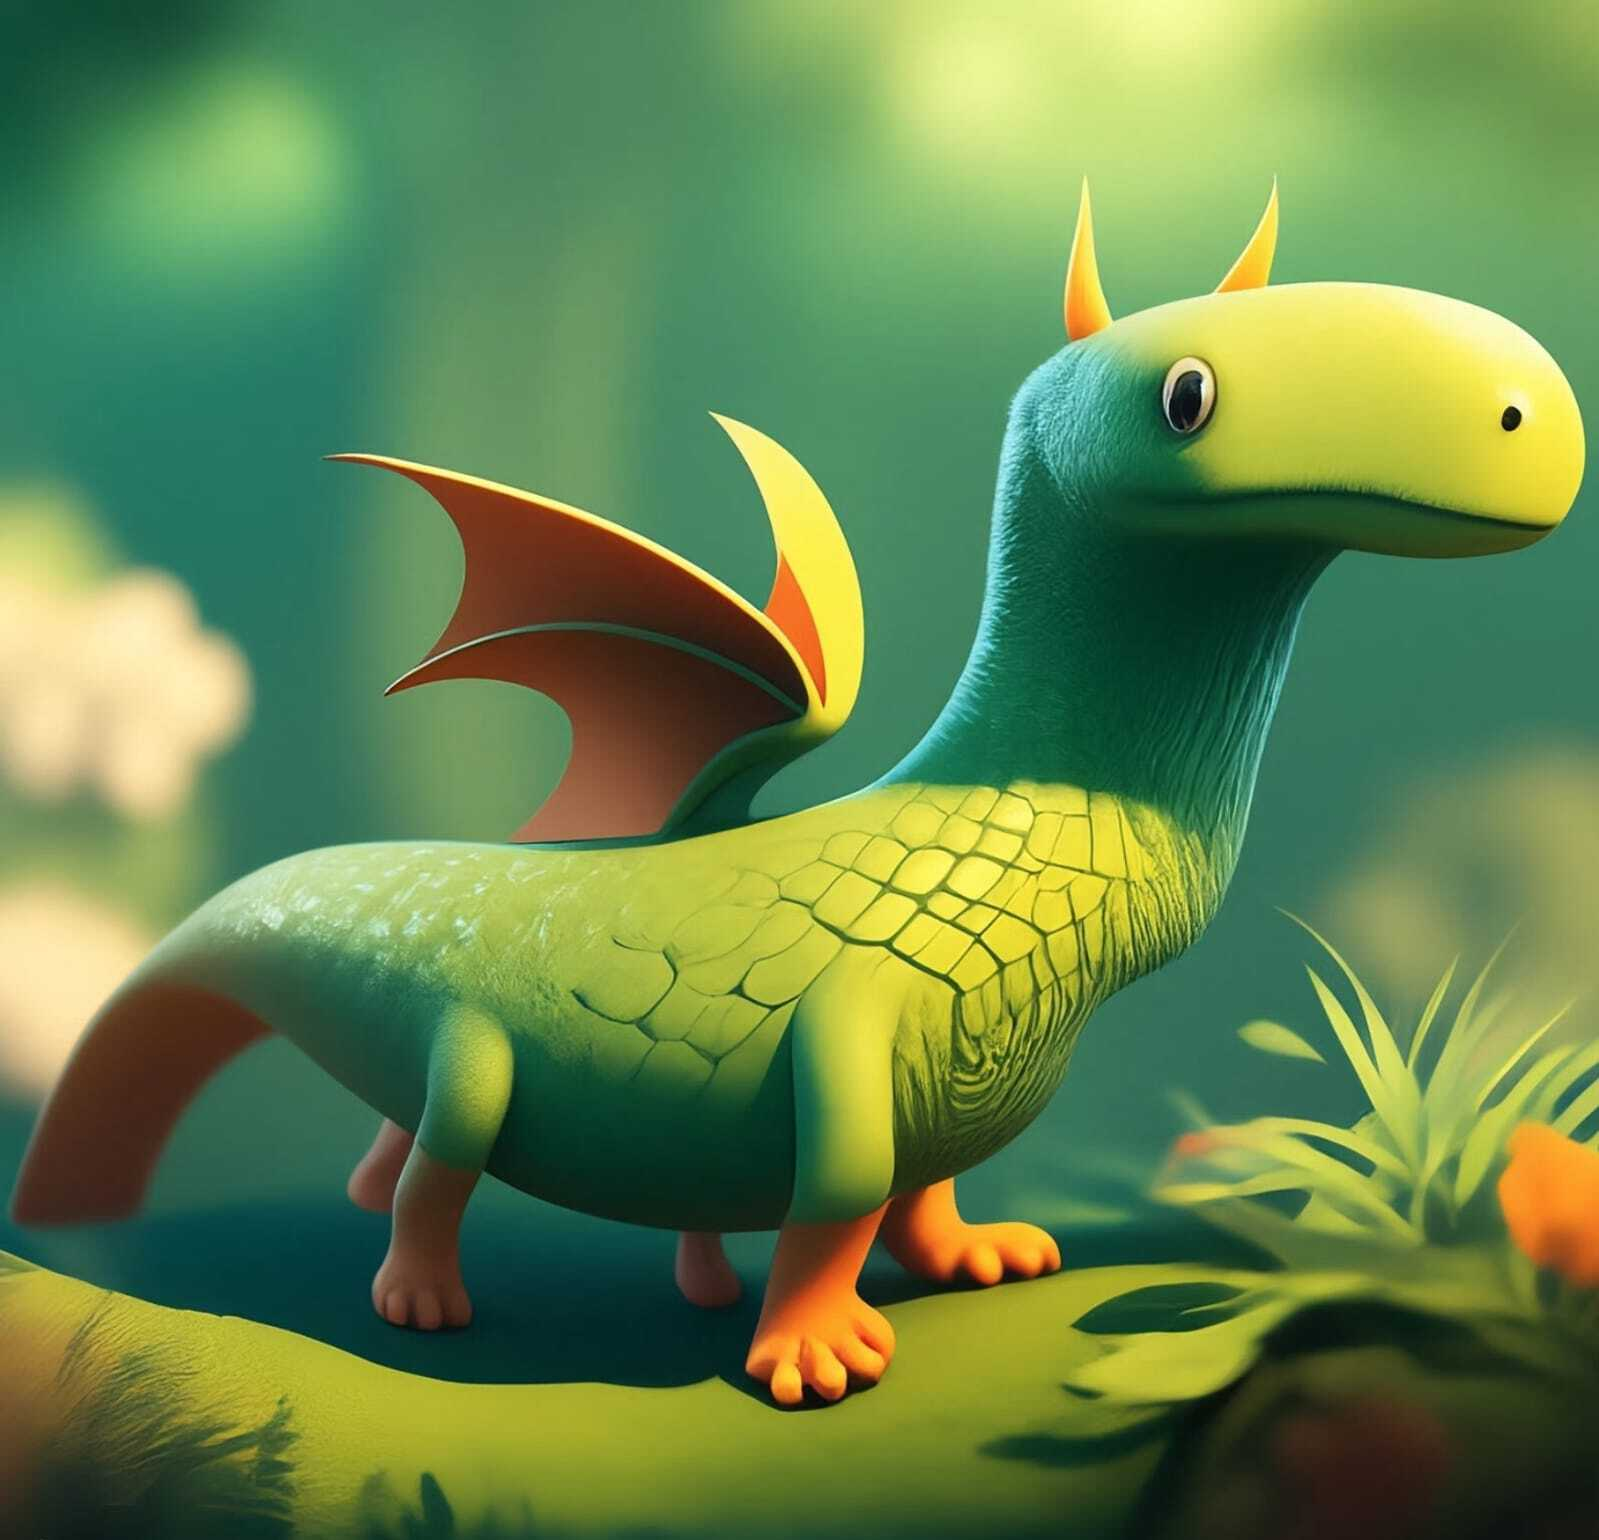
\includegraphics[width=6cm]{cover}
\end{center}
}

% theorem commands
\newtheoremstyle{c_remark}
	{}	% Space above
	{}	% Space below
	{}% Body font
	{}	% Indent amount
	{\bfseries}	% Theorem head font
	{}	% Punctuation after theorem head
	{.5em}	% Space after theorem head
	{\thmname{#1}\thmnumber{ #2}\thmnote{ \normalfont{\text{(#3)}}}}	% head content
\newtheoremstyle{c_definition}
	{3pt}	% Space above
	{3pt}	% Space below
	{}% Body font
	{}	% Indent amount
	{\bfseries}	% Theorem head font
	{}	% Punctuation after theorem head
	{.5em}	% Space after theorem head
	{\thmname{#1}\thmnumber{ #2}\thmnote{ \normalfont{\text{(#3)}}}}	% head content
\newtheoremstyle{c_plain}
	{3pt}	% Space above
	{3pt}	% Space below
	{\itshape}% Body font
	{}	% Indent amount
	{\bfseries}	% Theorem head font
	{}	% Punctuation after theorem head
	{.5em}	% Space after theorem head
	{\thmname{#1}\thmnumber{ #2}\thmnote{ \text{(#3)}}}	% head content

\ifcsname c@english\endcsname
	\theoremstyle{plain}
	\newtheorem{theorem}{Theorem}[section]
	\newtheorem{lemma}[theorem]{Lemma}
	\newtheorem{proposition}[theorem]{Proposition}
	\newtheorem*{proposition*}{Proposition}
	%\newtheorem{corollary}[theorem]{אין חלופה עברית}

	\theoremstyle{definition}
	\newtheorem{definition}[theorem]{Definition}
	\newtheorem*{definition*}{Definition}
	\newtheorem{example}{Example}[section]
	\newtheorem{exercise}{Exercise}[section]

	\theoremstyle{remark}
	\newtheorem*{remark}{Remark}
	\newtheorem*{solution}{Solution}
	\newtheorem{conclusion}[theorem]{Conclusion}
	\newtheorem{notation}[theorem]{Notation}
\else
	\theoremstyle{c_plain}
	\newtheorem{theorem}{משפט}[section]
	\newtheorem{lemma}[theorem]{למה}
	\newtheorem{proposition}[theorem]{טענה}
	\newtheorem*{proposition*}{טענה}
	%\newtheorem{corollary}[theorem]{אין חלופה עברית}

	\theoremstyle{c_definition}
	\newtheorem{definition}[theorem]{הגדרה}
	\newtheorem*{definition*}{הגדרה}
	\newtheorem{example}{דוגמה}[section]
	\newtheorem{exercise}{תרגיל}[section]

	\theoremstyle{c_remark}
	\newtheorem*{remark}{הערה}
	\newtheorem*{solution}{פתרון}
	\newtheorem{conclusion}[theorem]{מסקנה}
	\newtheorem{notation}[theorem]{סימון}
\fi

% Questions related commands
\newcounter{question}
\setcounter{question}{1}
\newcounter{sub_question}
\setcounter{sub_question}{1}

\ifcsname c@english\endcsname
	\newcommand{\question}[1][0]{
		\ifthenelse{#1 = 0}{}{\setcounter{question}{#1}}
		\section{Question \arabic{question}}
		\addtocounter{question}{1}
		\setcounter{sub_question}{1}
	}

	\newcommand{\subquestion}[1][0]{
		\ifthenelse{#1 = 0}{}{\setcounter{sub_question}{#1}}
		\subsection{Part \alph{sub_question}}
		\addtocounter{sub_question}{1}
	}
\else
	\newcommand{\question}[1][0]{
		\ifthenelse{#1 = 0}{}{\setcounter{question}{#1}}
		\section{שאלה \arabic{question}}
		\addtocounter{question}{1}
		\setcounter{sub_question}{1}
	}

	\newcommand{\subquestion}[1][0]{
		\ifthenelse{#1 = 0}{}{\setcounter{sub_question}{#1}}
		\subsection{סעיף \localecounter{letters.gershayim}{sub_question}}
		\addtocounter{sub_question}{1}
	}
\fi

% import lua and start of document
\directlua{common = require ('../common')}

\GetEnv{AUTHOR}

% headers
\author{\AUTHOR}
\date\today

\title{פתרון מטלה 06 --- מבנים אלגבריים (2), 80446}

\begin{document}
\maketitle
\maketitleprint[red]

\question{}
יהי $\xi_8 \in \CC$ שורש יחידה פרימיטיבי מסדר $8$. \\
נמצא את כל תתי־ההרחבות הריבועיות של $\QQ(\xi_8) / \QQ$,
כלומר את כל השדות $K$ כך ש־$\QQ \subseteq K \subseteq \QQ(\xi_8)$ ו־$[K : \QQ ] = 2$.
\begin{solution}
	נבחין כי מחישוב ישיר,
	\[
		\xi_8
		= e^{\frac{2\pi i}{8}}
		= \frac{1 + i}{\sqrt{2}}
	\]
	ולכן גם,
	\[
		\xi_8^3
		= \frac{-1 + i}{\sqrt{2}}
	\]
	ונסיק כי $\xi_8 - \xi_8^3 = \sqrt{2} \in \QQ(\xi_8)$.
	בנוסף מחיבור שני איברים אלה נסיק שגם $i \in \QQ(\xi_8)$.
	נסיק ש־$\QQ(\sqrt{2}, i) \subseteq \QQ(\xi_8)$, ונרצה להראות שוויון.
	אנו יודעים ש־$[\QQ(\sqrt{2}, i) : \QQ] = [\QQ(\sqrt{2}, i) : \QQ(\sqrt{2})] \cdot [\QQ(\sqrt{2}) : \QQ] = 4$.
	מצד שני גם $[\QQ(\xi_8) : \QQ] = [\QQ(\xi_8, \xi_8^2) : \QQ(\xi_8^2)] \cdot [\QQ(\xi_8^2) : \QQ] = 4$, כאשר השתמשנו בעובדה ש־$\xi_8^2 = \xi_4$ (מחישוב ישיר).
	נסיק אם כן שקיים שוויון דרגות ולכן בהכרח $\QQ(\xi_8) = \QQ(\sqrt{2}, i)$.

	עלינו אם כך למצוא את כל השדות $\QQ \subseteq K \subseteq \QQ(\sqrt{2}, i)$ מדרגה $2$ מעל $\QQ$, ונבחין כבר כמסקנה ש־$\QQ(i)$ וכן ש־$\QQ(\sqrt{2})$ מקיימים את הטענה.
	מבדיקה ישירה גם $\QQ(\sqrt{-2})$ הוא שדה כזה, ולא קיימים שדות נוספים כאלה, שכן שלושת האיברים הללו מרכיבים בסיס של $\QQ(\xi_8)$ לפי שאלה 3 ממטלה 3.
\end{solution}

\question{}
\subquestion{}
נוכיח את הזהויות הנתונות לפולינומים ציקלוטומיים.

\subsubsection{i}
נניח ש־$2 \nmid n$ ונוכיח,
$\Phi_{2n}(t) = \Phi_n(-t)$.
\begin{proof}
	\[
		t^{2n} - 1
		= \prod_{d \mid 2n} \Phi_d(t)
		= \prod_{d \mid n} \Phi_{2d}(t) \cdot \prod_{d \mid n} \Phi_d(t)
		= \prod_{d \mid n} \Phi_{2d}(t) \cdot (t^n - 1)
	\]
	ולכן,
	\[
		\prod_{d \mid n} \Phi_{2d}(t) = t^n + 1
	\]
	מצד שני,
	\[
		{(-t)}^n - 1
		= \prod_{d \mid n} \Phi_d(-t)
	\]
	אבל $2 \nmid n$ ולכן ${(-t)}^n - 1 = -(t^n + 1)$ ונסיק,
	\[
		\prod_{d \mid n} \Phi_{2d}(t)
		= - \prod_{d \mid n} \Phi_d(-t)
	\]
	ועתה נוכל להוכיח בפשטות את הטענה באינדוקציה על $n$, עבור $n = 1$ מתקיים,
	\[
		\Phi_2(t) = - \Phi_1(-t)
	\]
	עבור $n = 3$ בהתאם נובע,
	\[
		\Phi_{2}(t) \cdot \Phi_6(t)
		= - \Phi_1(-t) \cdot \Phi_3(-t)
	\]
	ומהמקרה $n = 1$ נסיק שהטענה חלה, עתה נניח שהטענה נכונה ל־$m < n$ ונבחן את $n$, נשתמש בתהליך דומה למקרה $n = 3$ ונבטל את המכפלות הקטנות, נובע ישירות,
	\[
		\Phi_{2n}(t)
		= \Phi_n(-t)
	\]
	והשלמנו את המהלך.
\end{proof}

\subsubsection{ii}
נניח ש־$p$ ראשוני ונראה ש־$\Phi_{pn}(t) = \Phi_n(t^p)$ אם $p \mid n$, ואחרת $\Phi_{pn}(t) = \Phi_n(t^p) / \Phi_n(t)$.
\begin{proof}
	אנו יודעים כי $\mu_{pn}$ חבורה ציקלית, ולכן $\zeta \in \mu_{np}$ אם ורק אם $\zeta^p \in \mu_n$, זאת ישירות מטעמי דרגה. \\
	נסיק ש־$t - \zeta \mid \Phi_{pn}(t)$ אם וקר אם $t - \zeta^p \mid \Phi_{n}(t^p)$ ישירות מהגדרת $\Phi$.
\end{proof}

\subquestion{}
נחשב את $\Phi_n(t)$ עבור $1 \le n \le 10$.
\begin{solution}
	עבור $n = 1$ אנו יודעים כי $\Phi_1(t) = t - 1$ ישירות מהגדרה.
	אנו גם יודעים ש־$\Phi_2(t) = \frac{t^2 - 1}{t - 1} = t + 1$.
	עבור $n = 3, 5, 7$ נשתמש בעובדה שהם ראשוניים ולכן,
	\[
		\Phi_p(t) = \frac{t^n - 1}{t - 1}
	\]
	ונקבל $\Phi_3(t) = t^2 + t + 1, \Phi_5(t) = t^4 + t^3 + t^2 + t + 1, \Phi_7(t) = t^6 + t^5 + t^4 + t^3 + t^2 + t + 1$. \\
	עבור $n = 4$ נשתמש בעובדה ש־$\Phi_{2 \cdot 2}(t) = \Phi_2(t^2)$ מתת־הסעיף הקודם ונובע ש־$\Phi_4(t) = t^2 + 1$.
	עבור $n = 6$ נקבל מתת־הסעיף הראשון $\Phi_6(t) = \Phi_3(-t) = t^2 - t + 1$.
	עבור $n = 8$,
	\[
		t^8 - 1
		= \prod_{d \mid 8} \Phi_d(t)
		\iff
		\Phi_8(t)
		= \frac{t^8 - 1}{(t - 1)(t + 1)(t^2 - 1)}
		= t^4 + 1
	\]
	וכך גם,
	\[
		\Phi_9(t)
		= \Phi_3(t^3)
		= t^6 + t^3 + 1
	\]
	ולבסוף,
	\[
		\Phi_{10}(t)
		= \Phi_5(-t)
		= t^4 - t^3 + t^2 - t + 1
	\]
\end{solution}

\question{}
ראינו כי $\FF_{p^d} / \FF_p$ היא הרחבה ציקלוטומית על־ידי שורש יחידה $\xi$ מסדר $p^d - 1$. \\
ראינו גם כי במקרה זה יש שיכון $\aut(\FF_{p^d} / \FF_p) \hookrightarrow \aut(\mu_{p^d - 1}) \simeq {(\ZZ / (p^d - 1) \ZZ)}^\times$. \\
אנו נתאר את השיכון,
\[
	\aut_{\FF_p}(\FF_{p^d})
	= \operatorname{Fr}_p^{\ZZ / d \ZZ}
	\hookrightarrow {(\ZZ / (p^d - 1) \ZZ)}^\times
\]
נבדוק מה היא תמונת איבר פרוביניוס $\operatorname{Fr}_p$.
\begin{solution}
	נראה כי $\aut_{\FF_p}(\FF_{p^d}) \hookrightarrow \aut(\FF_{p^d} / \FF_p)$.
	יהי $\sigma = \operatorname{Fr}_p^n \in \aut_{\FF_p}(\FF_{p^d})$,
	אנו כבר יודעים כי זוהי חבורה ציקלית ובחרנו את אחד מאיבריה.
	נבחר $\tau \in \aut(\FF_{p^d} / \FF_p)$ על־ידי $\tau(x) = \sigma(x) / \FF_p$.
	נבחין כי מהגדרה כל $\sigma, \sigma'$ כאלה מסכימות על $\FF_p$, כלומר $\sigma \restriction \FF_p = \sigma' \restriction \FF_p$ ולכן $\tau = \tau'$ אם ורק אם $\sigma = \sigma'$, וזהו אכן שיכון.
	נבחין כי $\xi \mapsto \xi^{p^n}$ ב־$\tau$ על־פי ההגדרה, וזהו שיכון $\varphi \in \aut(\mu_{p^d - 1})$ מהגדרת $\xi$, וכן $\varphi \mapsto \phi$ עבור $\phi(m) = m \cdot p^n$,
	כפי שהגדרנו את האיזומורפיזם $\aut(\mu_{p^d - 1}) \simeq {(\ZZ / (p^d - 1) \ZZ)}^\times$.
	כלומר $\operatorname{Fr}_p^n \mapsto (m \mapsto m \cdot p^n)$ לכל $\operatorname{Fr}_p^n \in \aut_{\FF_p}(\FF_{p^d})$.

	בפרט נוכל להסיק שעבור $n = 1$ מתקבל $m \mapsto p m$.
\end{solution}

\question{}
תהי $q = p^k$ חזקת ראשוני.
פולינום $f \in \FF_q[x]$ מדרגה $d > 1$ נקרא פרימיטיבי אם הוא אי־פריק וכל שורש של $f$ ב־$\FF_{q^d}$ הוא יוצר של $\FF_{q^d}^\times$.

\subquestion{}
נמצא דוגמה לשדה סופי ולפולינום אי־פריק מדרגה $d > 1$ מעל $\FF_q$ שאינו פרימיטיבי.
\begin{solution}
	נגדיר $p = 3, k = 1$ ואת הפולינום $f(x) = x^2 + 1$, מבדיקה ישירה נקבל ש־$f$ אי־פריק ב־$\FF_3$. \\
	$d = \deg_{\FF_3} f = 2$ ולכן נבחן את שורשי $f$ ב־$\FF_9$. \\
	נגדיר $\FF_9 = \FF_3(\xi)$ עבור $\xi$ שורש יחידה פרימיטיבי מסדר $p^d - 1 = 8$, ונסיק ש־$f(x) = (x - \xi^4)(x - 2 \xi^4)$. \\
	נבחין כי $|\langle \xi^4 \rangle| = |\langle 2\xi^4 \rangle| = 3$ בעוד $|\FF_{q^d}^\times| = 8$ ולכן פולינום זה לא פרימיטיבי.
\end{solution}

\subquestion{}
נראה שאם $\alpha \in \FF_{q^d}$ יוצר את $\FF_{q^d}^\times$ אז המסלול שלו ב־$\aut(\FF_{q^d} / \FF_q)$ מכיל $d$ איברים שונים.
\begin{proof}
	$|\FF_{q^d}^\times| = q^d - 1$ שכן כל איבר לא טריוויאלי הוא הפיך. \\
	יהי $\zeta^n \in \FF_{q^d}^\times = {\FF_{q}(\zeta)}^\times$ עבור $\zeta$ שורש יחידה פרימיטיבי מסדר $q^d - 1$, כאשר $n \in \ZZ / (q^d - 1) \ZZ$.
	$\zeta \mapsto \zeta^n$ הוא אוטומורפיזם ולכן בפרט משרה $\sigma \in \aut(\FF_{q^d} / \FF_q)$ על־ידי $\pi(\zeta) = \pi(\zeta^n)$.
	נתון לנו שלכל $n$, קיים $m$ כך ש־$\alpha^m = \zeta^n$ ולכן נוכל להסיק ישירות שקיים $\sigma$ כך ש־$\sigma(\pi(\alpha)) = \pi(\zeta^n)$,
	כלומר גודל המסלול של $\alpha$ ב־$\aut(\FF_{q^d} / \FF_q)$ הוא $\varphi(q^d - 1) \ge d$.
\end{proof}

\subquestion{}
נוכיח שיש בדיוק $\varphi(q^d - 1) / d$ פולינומים פרימיטיביים מתוקנים מדרגה $d$ ב־$\FF_q[x]$.
\begin{proof}
	משאלה 3 ומהסעיף הקודם נוכל להסיק שיש $\varphi(q^d - 1)$ איברים שונים שיוצרים את $\FF_{q^d}^\times$,
	זאת על־ידי בחינת השיכון ב־$\ZZ / (q^d - 1) \ZZ$.
	אילו $f, g \in \FF_q[x]$ שני פולינומים שונים כך ש־$f(\xi) = g(\xi) = 0$ עבור $\xi$ יוצר של $\FF_q^\times$, אז נקבל שקיים $h \mid f, g$ פולינום פרימיטיבי מדרגה קטנה מ־$d$.
	אבל נקבל ש־$\FF_q / (h) \simeq \FF_{q^d}$ בסתירה לדרגת $h$, ולכן לא קיימים פולינומים כאלה.
	בנוסף השורשים הם שונים כמסקנה ממשפט 5.5.11, ולכן נסיק מכמות האיברים שחייבים להיות בדיוק $\frac{\varphi(q^d - 1)}{d}$ פולינומים כאלה.
\end{proof}

\end{document}
